

\documentclass{article}
\usepackage{hyperref}
\usepackage[utf8]{inputenc}
\usepackage{graphicx}
\usepackage{ragged2e}
\usepackage{listings}
\usepackage{xcolor}
\usepackage{colortbl}
\usepackage{color}
\usepackage{array}
\usepackage{csvsimple}

\lstset { %
    language=C,
    backgroundcolor=\color{black!5}, % set backgroundcolor
    basicstyle=\footnotesize,% basic font setting
}
 
\begin{document}

\begin{titlepage}
	\centering
	\vspace{1cm}
	{\scshape\Large PAR Laboratory Assignment\par}
	\vspace{0.75cm}
	{\Large Course 2018/19 (Fall semester)\par}
	\vspace{0.75cm}
	{\huge\bfseries Lab 2:  Embarrassingly parallelism with OpenMP: Mandelbrot set\par}
	\vspace{1cm}
	{\Large\itshape Pablo Vizcaino, Guillem Ramírez\par}
    \vspace{0.5cm}
    {\Large User: Par2206\par}
    \vfill
% Bottom of the page
	{\large \today\par}
\end{titlepage}

 
\clearpage
\tableofcontents
\clearpage 

\section{Introduction}
\justify
In this laboratory we are going to study the task decomposition and the parallelization strategies of the computation of the Mandelbrot set.


\justify
The Mandelbrot set is a set of complex numbers \textit{C} obtained from iterating the equation $Z = z^2 + C$.
You can see a visualization of the result from the computation in the figure \ref{fig:mandelbrot1}


\begin{figure}[ht]
    \centering
    
\includegraphics[width=0.75\textwidth]{mandelbrot.jpg}
    \caption{Mandelbrot visualization}
    \label{fig:mandelbrot1}
\end{figure}
\newpage
\section{Parallelization strategies analysis}
\justify
Our first objective is to analyze the data dependency within the Mandelbrot computation. With this purpose we decided to explore row and point granularity. All executions with tareador use the option -w 8, which means 8 iterations per loop.

\subsection{Point decomposition}
In this section we are presenting the point decomposition strategy , where we are creating at each inner loop iteration a task.
\subsubsection*{Point decomposition analysis with \textit{tareador}}
We just needed to add tareador start task directive in the beginning of the inner for loop and a tareador end task at the end of the inner for loop. You can find the source code at \textit{code/tareador/mandel-tar-point.c}. Listing \ref{code:tareadorPoint} shows the structure.

\begin{lstlisting}[caption={Tareador instrumentation at point granularity},label=code:tareadorPoint]
    /* Calculate points and save/display */
    for (row = 0; row < height; ++row) {
        for (col = 0; col < width; ++col) {
            tareador_start_task("point");
                        .
                        .
                        .
            tareador_end_task("point"); 
\end{lstlisting}

\justify
The result obtained from executing \textit{run-tareador.sh} with \textit{mandel-tar} objective (non-graphical version) is:

\begin{figure}[ht]
    \centering
    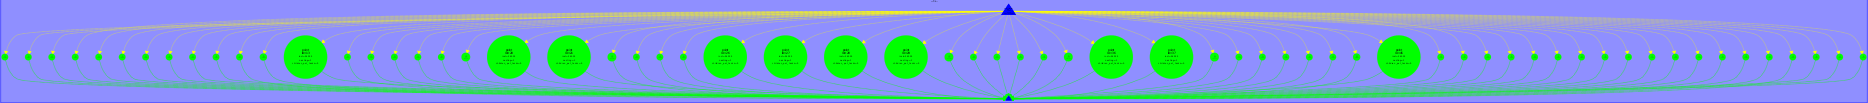
\includegraphics[width=1\textwidth]{mandel-tar-point-graph.png}
    \caption{Tareador graph with point granularity}
    \label{fig:tareadorpoint}
\end{figure}
\justify
From the graph obtained we can observe that there are 64 non-dependant tasks, one for each point: $64 == 8*8$. 
Due to the big number of tasks the graph is in a long shape, you can view the source image at \textit{img/tareador/mandel-tar-point-graph.png}. From the graph we can conclude that working with a big number of tasks can carry out to overheads. 

\newpage
\subsection{Row decomposition}
\label{sec:rowAnalysis}
In this section we are presenting the row decomposition strategy, where we are creating a task for each row of points. 
\subsubsection*{Row decomposition analysis with \textit{tareador}}
For this analysis we just need to add tareador directives in the middle of the for loops. You can find the source code at \textit{code/tareador/mandel-tar-row.c}. Listing \ref{code:tareadorRow} shows the structure.

\begin{lstlisting}[caption={Tareador instrumentation at row granularity},label=code:tareadorRow]
    /* Calculate points and save/display */
    for (row = 0; row < height; ++row) {
        tareador_start_task("row");
        for (col = 0; col < width; ++col) {
                    .
                    .
                    .
        }
        tareador_end_task("row");       
    }
\end{lstlisting}
\justify
The result from executing \textit{run-tareador.sh} with \textit{mandel-tar} objective (non-graphical version) is:
\begin{figure}[h]
    \centering
    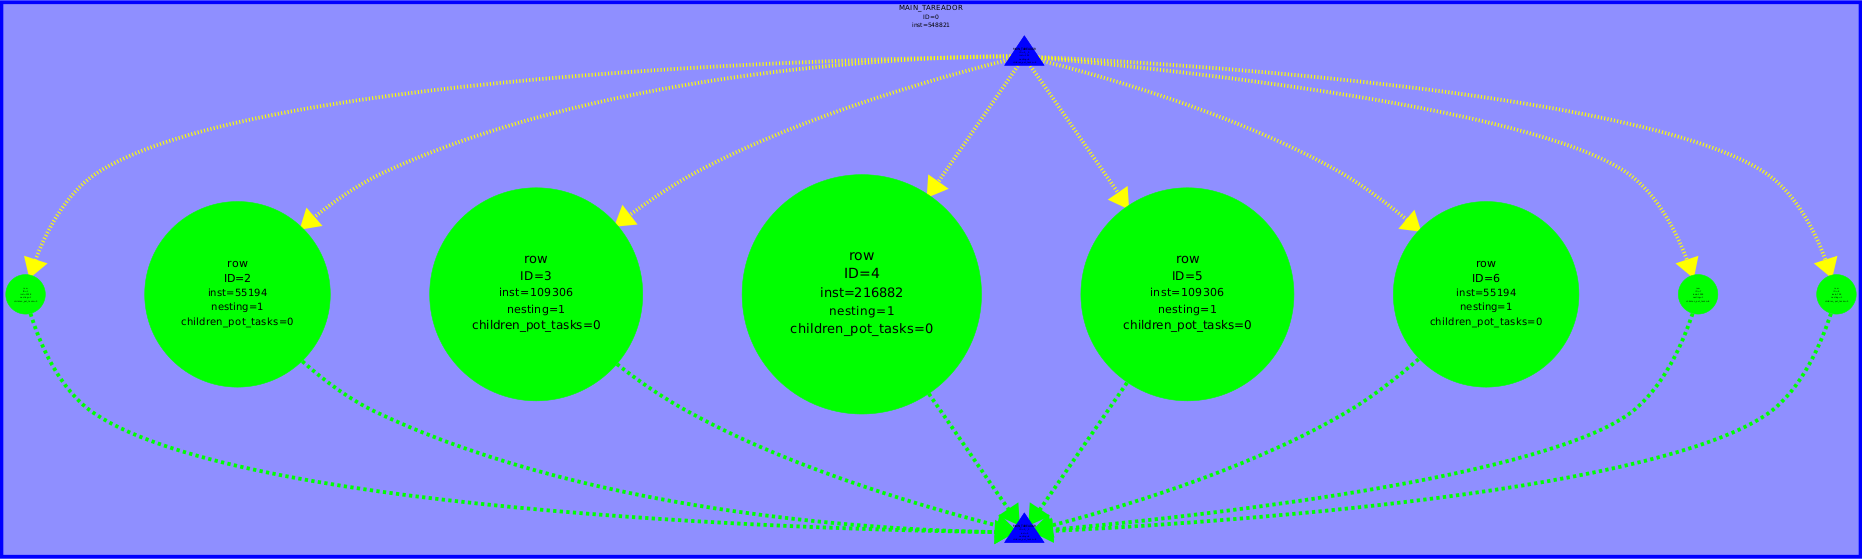
\includegraphics[width=0.99\textwidth]{mandel-tar-row-graph.png}
    \caption{Tareador graph with row granularity}
    \label{fig:tareadorrow}
\end{figure}

\justify
From the graph we can observe that we get 8 non-dependant tasks, one for each row, as expected. With less tasks we may have less overheads from the previous version but we may not be taking profit of all threads. This question will be evaluated in the following sections. The source image is at \textit{img/tareador/mandel-tar-row-graph.png}. 

\newpage
\subsection{Preliminary comparison between strategies}
\justify
After analyzing the two versions we find out that with a point based strategy the number of tasks is: $w^2$ . In our case w is 8 so the number of tasks is 64, this number can increase to really high values in default executions and can be really problematic due to task creation and work distribution overheads. In the other hand we find out that row granularity the number of task linearly increase with w, which may be a more affordable value. This general guidelines and ideas will be taken into account for the next sections.

 \subsection{Graphical version analysis}
\label{sec:graphical}
\justify
Once the granularity of the computation itself is evaluated, we will be analyzing the graphical version. For this purpose we will be using the same source code as in the previous subsection (\textit{code/tareador/mandel-tar-row.c}) but we will be compiling using the \textit{mandeld-tar} Makefile target. 


\begin{figure}[ht]
    \centering
    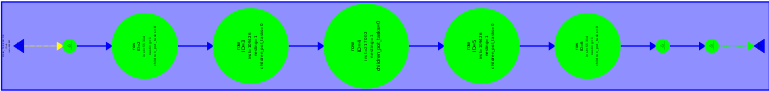
\includegraphics[width=0.99\textwidth]{r-mandeld.png}
    \caption{Tareador graph with mandeld target}
    \label{fig:tareadormandeld}
\end{figure}

\justify
The image is rotated for document structuring purpose. The full non-rotated image can be found in \textit{img/tareador/mandeld-tar.png}.

\justify
We can observe that due to dependencies the graph is now serialized, if we look into the edges between tasks in tareador we can see that a graphics library variable is now needed between iterations. This is causing the serialization of the graph.

\begin{figure}[h]
    \centering
    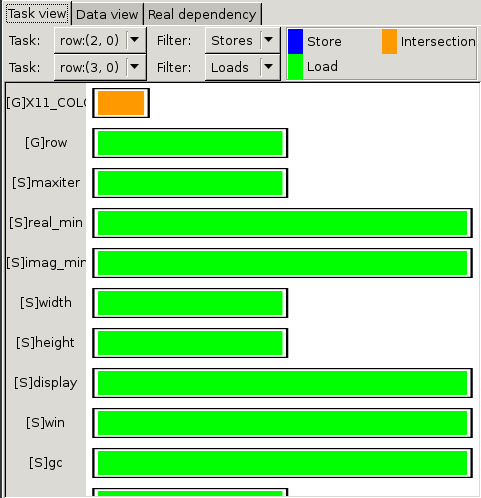
\includegraphics[width=0.32\textwidth]{mandeld-tar-edge.png}
    \caption{Variable usage between tasks}
    \label{fig:mandeldtaredge}
\end{figure}
\justify
If we look into the code we can find that the the part causing serialization of the task graph is:

\begin{lstlisting}
    #if _DISPLAY_
            /* Scale color and display point  */
            long color = (long) ((k-1) * scale_color) + min_color;
            if (setup_return == EXIT_SUCCESS) {
                XSetForeground (display, gc, color);
                XDrawPoint (display, win, gc, col, row);
            }
    #else
\end{lstlisting}
\justify
Specially what is causing serialization is the inner if statement. In the following sections we will be parallelizing the code, for protecting this part we will be adding the following clause before the if statement so that we are telling openMP that only one thread can be working at any time.

\begin{lstlisting}
    #pragman omp critical
    if (setup_return == EXIT_SUCCESS) {
\end{lstlisting}
\newpage
\section{Parallelization strategies implementation}
In this section we are going to present the implementation of both strategies in \textit{OpenMP}
\subsection{Point decomposition in \textit{OpenMP}}
For this strategy we went through a few versions. Starting with the initial version and making improvements.
\subsubsection*{Initial version}
The initial version was given in the assignment and its:
\begin{lstlisting}
    for (row = 0; row < height; ++row) {
        #pragma omp parallel
        #pragma omp single
        for (col = 0; col < width; ++col) {
            #pragma omp task firstprivate(col)

\end{lstlisting}
\justify
In this version we introduced the firsprivate pragma which tells the compiler that the col variable inside the construct is a new variable initialized to the same original variable value.

\justify
Also notate that in the full code \textit{code/omp/mandel-omp-initial.c} we added the \textit{\#pragma omp critical} clause in the region that generated dependencies, see: \hyperref[sec:graphical]{\textit{graphical version analysis}}.


\begin{figure}[h]
    \centering
    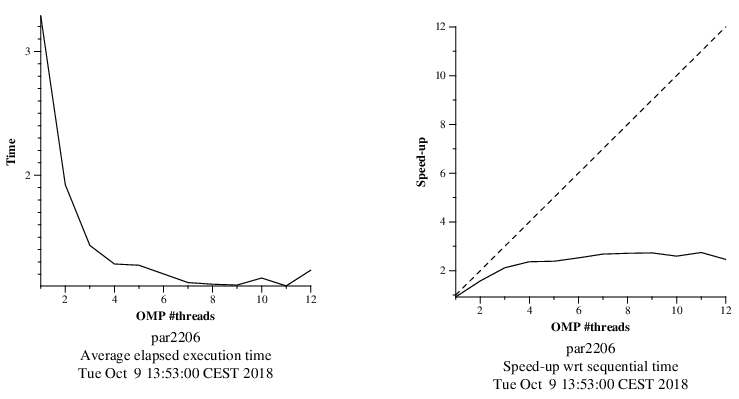
\includegraphics[width=1\textwidth]{strongPoint.png}
    \caption{Strong scalability plots for initial version}
    \label{fig:strongpoint}
\end{figure}
\justify
We can observe that the speedup poorly improves with the increase of \#threads that's due to the version not being optimized as we create a lot of tasks and the work distribution takes into serious overheads. We can evaluate the overheads measuring in paraver the number of bursts (in this case, 800)

\subsubsection*{Improved version}
In this version we move out the loop \textit{parallel and single pragmas} and in consequence we also privatize the row variable.

\begin{lstlisting}
    #pragma omp parallel
    #pragma omp single
    /* Calculate points and save/display */
    for (int row = 0; row < height; ++row) {
        for (int col = 0; col < width; ++col) {
            #pragma omp task firstprivate(row, col)

\end{lstlisting}
In this version, as we move the parallel region and the work-distribution outside the loop we don't invoke it at each iteration of row, so we only do it once. This slightly improves the performance as you can see in the strong scalability plots.
\begin{figure}[h]
    \centering
    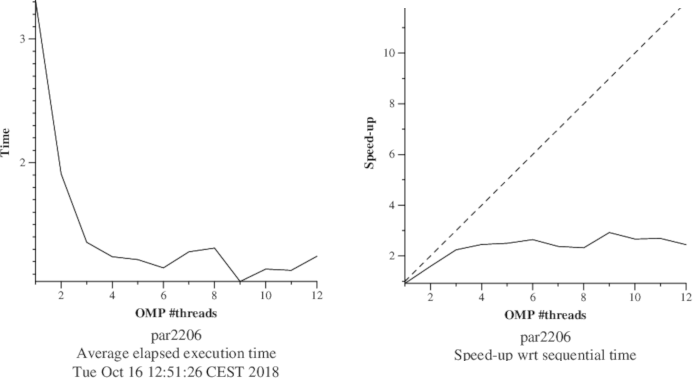
\includegraphics[width=1\textwidth]{strongPoint2.png}
    \caption{Strong scalability plots for the improved version}
    \label{fig:strongpoint2}
\end{figure}

\subsubsection*{Taskloop version}   
\justify
In this version we introduce the taskloop pragma. This statement distributes more efficiently each task's work in a loop. Nonetheless, it creates and implicit taskgroup barrier. Since we observed that all iterations are independent, there is no need for synchronizations. To remove them we added a \textit{nogroup} clause.


\begin{lstlisting}
    #pragma omp parallel
    #pragma omp single
    /* Calculate points and save/display */
    for (int row = 0; row < height; ++row) {
        #pragma omp taskloop firstprivate(row) num_tasks(width) \
        nogroup
        for (int col = 0; col < width; ++col) {
\end{lstlisting}
\justify
If we look the strong scalability plots and we compare them to the previous ones we can see how big the improvement is. This is due to the optimization in the task creation and distribution and also in the elimination of the barrier.

\begin{figure}[h]
    \centering
    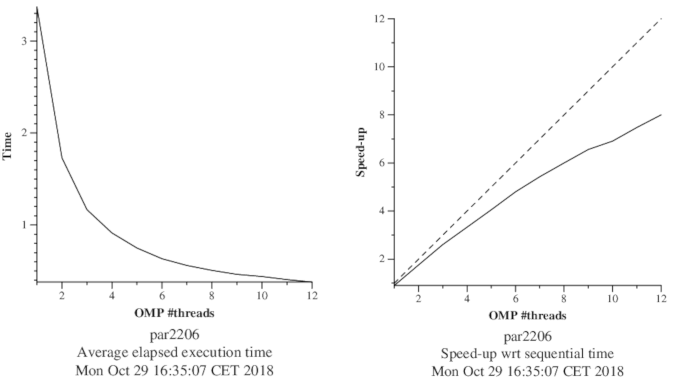
\includegraphics[width=1\textwidth]{strongPoint3.png}
    \caption{Strong scalability plots for the taskloop version}
    \label{fig:strongpoint3}
\end{figure}
\subsection{Row decomposition in \textit{openMP}}
\justify
In this section we implemented the row decomposition, which we analyzed in section: \hyperref[sec:rowAnalysis]{\textit{Row decomposition}}

\justify
As we observed in the previous sections, reducing overheads is the key to a better performance; so we expect to reduce the execution time when we reduce the granularity to one task for each row.\newline You can find the full code at \textit{code/omp/mandel-omp-row.c}. Here you have the pragma setup:

\begin{lstlisting}
    #pragma omp parallel
    #pragma omp single
    /* Calculate points and save/display */

   #pragma omp taskloop num_tasks(height) nogroup 
    for (int row = 0; row < height; ++row) {
        for (int col = 0; col < width; ++col) {
\end{lstlisting}
\justify
To achieve row granularity, we placed the pragma outside both loops, and used the clause num\_tasks(height) to set the granularity to one task per row. We also kept the nogroup clause to eliminate the implicit barrier.  


\begin{figure}[h]
    \centering
    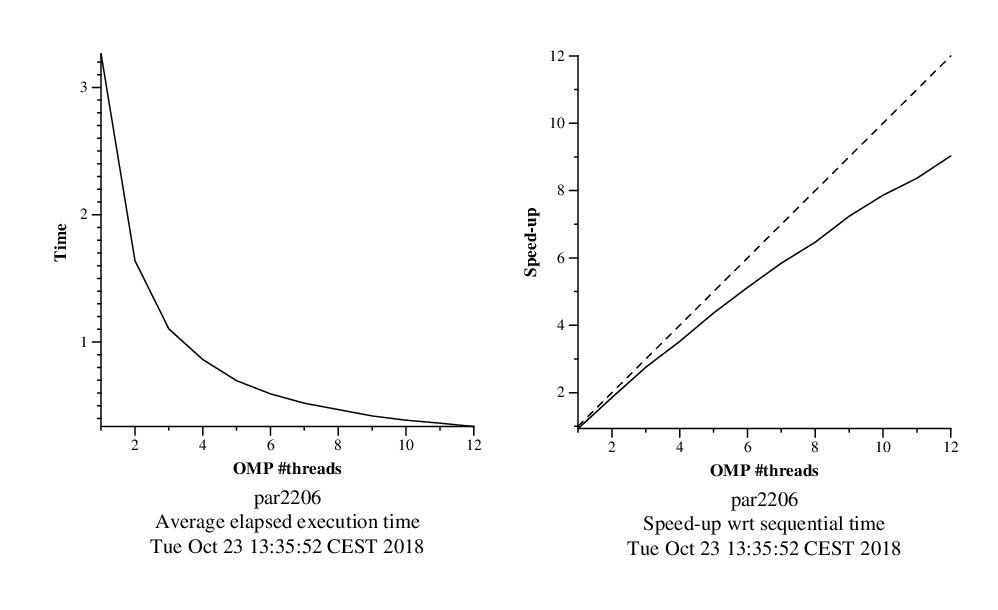
\includegraphics[width=1\textwidth]{strongRow.png}
    \caption{Strong scalability plots for the Row-Granularity version}
    \label{fig:strongrow}
\end{figure}

\justify
As can be seen in the Figure \ref{fig:strongrow} the strong scalability has slightly improved compared to the previous versions. This fulfills our expectations. In the following section we will be comparing the execution times to confirm this improvement. 
\justify
We also tried to change the granularity (p.e: one task each to rows) modifying the num\_tasks clause and as you can see in the following figure the reduction of overheads doesn't compensate the loss in parallelization. Notice that this is the opposite behaviour than in the point version. This is due to, the smaller the granularity in the point version, the more similar to the row one it is. 


\begin{table}[h!]
\centering
\begin{tabular}{|r|r|r|r|}
\hline
\multicolumn{2}{|l}{Point}                                    & \multicolumn{1}{|l}{Row}       & \multicolumn{1}{l|}{}          \\ \hline
\multicolumn{1}{|l|}{Tasks/row} & \multicolumn{1}{l|}{Time (s)} & \multicolumn{1}{l|}{Tasks/col} & \multicolumn{1}{l|}{Time (s)}  \\ \hline
800                           & 0.513                        & 800                           & 0.47                          \\ \hline
400                           & 0.474                        & 400                           & 0.485                         \\ \hline
200                           & 0.481                        & 200                           & 0.489                         \\ \hline
100                           & 0.474                        & 100                           & 0.509                         \\ \hline
50                            & 0.488                        & 50                            & 0.524                         \\ \hline
25                            & 0.47                         & 25                            & 0.673                         \\ \hline
5                             & 0.451                        & 5                             & 2.515                         \\ \hline
1                             & 0.46                         & 1                             & 3.481  \\ \hline                   
\end{tabular}
\end{table}


\newpage
\section{Performance evaluation}
\justify
When obtaining the execution times of both versions with default parameters we get \textit{0.51 s} for the point granularity and \textit{0.47 s} for the row granularity.
To observe better the difference, we also executed both versions with \textit{maxiter} variable equal to 300000. The results obtained with this parameter are \textit{95.09 s} for the point version and \textit{13.02 s} for the row version. We can see that as we increase the problem size the time difference is more noticeable.
\justify 
First we are going to evaluate the percentage of time that each version wastes on task creation and synchronizations. We executed point and row version (both with no group) with paraver instrumentation and used omp\_tasks configuration file. We can see in the following table that for each thread the time consumed by the overheads in the point version is greater than in the row one. In consequence, in the row version, threads spends more time calculating and the execution time is lower. 
\begin{table}[h!]
\arrayrulecolor{black}
\begin{tabular}{!{\color{black}\vrule}l!{\color{black}\vrule}r!{\color{black}\vrule}r!{\color{black}\vrule}r!{\color{black}\vrule}r!{\color{black}\vrule}} 
\cline{2-5}
\multicolumn{1}{l!{\color{black}\vrule}}{} & \multicolumn{2}{l!{\color{black}\vrule}}{Row strategy}                                                                  & \multicolumn{2}{l!{\color{black}\vrule}}{Point strategy}                                                                 \\ 
\cline{2-5}
\multicolumn{1}{l!{\color{black}\vrule}}{} & \multicolumn{1}{l!{\color{black}\vrule}}{Code exectuing} & \multicolumn{1}{l!{\color{black}\vrule}}{Taskloop construct} & \multicolumn{1}{l!{\color{black}\vrule}}{Code executing} & \multicolumn{1}{l!{\color{black}\vrule}}{Taskloop construct}  \\ 
\hline
THREAD 1.1.1                               & 99.97                                                    & 0.03                                                         & 97.55                                                    & 2.45                                                          \\ 
\hline
THREAD 1.1.2                               & 99.9                                                     & 0.1                                                          & 97.45                                                    & 2.55                                                          \\ 
\hline
THREAD 1.1.3                               & 99.8                                                     & 0.2                                                          & 98.99                                                    & 1.01                                                          \\ 
\hline
THREAD 1.1.4                               & 99.81                                                    & 0.19                                                         & 97.58                                                    & 2.42                                                          \\ 
\hline
THREAD 1.1.5                               & 99.97                                                    & 0.03                                                         & 97.5                                                     & 2.5                                                           \\ 
\hline
THREAD 1.1.6                               & 99.98                                                    & 0.02                                                         & 97.63                                                    & 2.37                                                          \\ 
\hline
THREAD 1.1.7                               & 100                                                      & 0                                                            & 97.37                                                    & 2.63                                                          \\ 
\hline
THREAD 1.1.8                               & 99.99                                                    & 0.01                                                         & 97.33                                                    & 2.67                                                          \\ 
\hline
\multicolumn{1}{l}{}                       & \multicolumn{1}{l}{}                                     & \multicolumn{1}{l}{}                                         & \multicolumn{1}{l}{}                                     & \multicolumn{1}{l}{}                                          \\ 
\hline
Average                                    & 99.93                                                    & 0.08                                                         & 97.68                                                    & 2.32                                                          \\
\hline
\end{tabular}
\arrayrulecolor{black}
\end{table}

\iffalse
\begin{figure}[h]
    \centering
    \includegraphics[width=1\textwidth]{percentRowPoint.png}
    \caption{Comparison between row and point strategy percentage time of code executing and overheads.}
    \label{fig:rowpointpercent}
\end{figure}
\fi
\newpage
\section{Conclusions}
\justify
In this lab assignment we understand the importance of the work-distribution and task creation overheads in the parallelization process. We saw that the best result is obtained when there is a balance between parallelization and the reduction of overheads.It's important to set the grain size properly to optimize the execution time, because it affects directly to the parallelization and the overheads.

\justify
We also learned the different \textit{OpenMP} pragmas that we can use to parallelize loop-based codes and to set different grainsize and control the barriers and synchronizations.

\justify
Another key factor that helped us to compare different versions and to confirm the results that we were expecting is the \textit{Paraver} instrumented execution of the codes. 
\end{document}

    